\documentclass[12pt]{beamer}
\usetheme[dept=ai,coloredtitles,coloredblocks,showsection,copyright={Paper under review}]{vub} % This will automatically load all fonts (Roboto and TeX Gyre Adventor
               % for titles), and the VUB colors. Also includes the triangle.
\title{Step-wise explanations of constraint satisfaction problems (ZebraTutor)}
% \department{ai}
%\subtitle{Your subtitle} % Can be omitted
\usepackage{graphicx}
\usepackage{amsmath}
\usepackage{amssymb}
\usepackage{amssymb}
\author{{\bf Bart Bogaerts} \and Emilio Gamba \and Jens Claes \and Tias Guns}

% …

\begin{document}
\frame{\maketitle} % Automatic titlepage with VUB logo.

\begin{frame}{Motivation}
\begin{itemize}
 \item Our take on \emph{explainable AI}
 \item Context: Constraint solving
 \item Explain (strong, complex) propagation in simple steps
 \item Interactive constraint solving
\end{itemize}

\end{frame}

\begin{frame}{History}
\begin{itemize}
 \item 2019 Holy Grail Challenge: Zebra puzzles
 \begin{itemize}
    \item Parse puzzles and translate into CSP
    \item Solve CSP automatically
    \item Explain in a human-understandable way how to solve this puzzle
 \end{itemize}
 \item More generic paper under review for ECAI 2020
\end{itemize}

 
\end{frame}


\begin{frame}{Contributions}
\begin{itemize}
 \item Formalize the step-wise explanation problem
 \item Propose an algorithm (agnostic of actual propagators, consistency level, etc.)
 \item Propose heuristics for guiding the search for explanations
 \item Experimentally demonstrate feasibility
\end{itemize}
 
\end{frame}


\begin{frame}{Logic Grid Puzzles}
 \begin{itemize}
  \item Set of clues
  \item Sets of entities that need to be linked
  \item Each entitity is linked to exactly one entity of each other type
  \item The links are consistent (transitivity)
 \end{itemize}

\end{frame}

\begin{frame}{Logic Grid Puzzles}\centering
\hspace*{-30pt}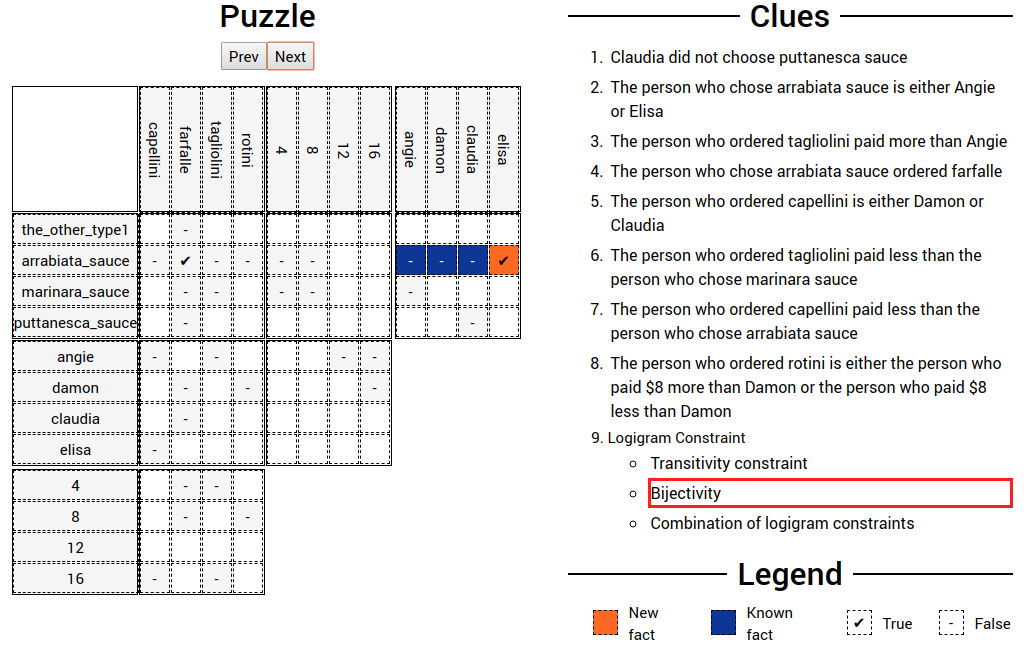
\includegraphics[width=1.2\textwidth]{zebra_screen.png} 
 \end{frame}
% \end{frame}

\begin{frame}{Problem}
 \begin{definition}
 Let $I_{i-1}$ and $I_i$ be partial interpretations such that $I_{i-1}\wedge T \models I_i$.
 We say that $(E_i,S_i,N_i)$ \emph{explains} the derivation of $I_{i}$ from $I_{i-1}$ if the following hold:
\begin{itemize}
    \item $N_i= I_i \setminus I_{i-1}$ (i.e., $N_i$ consists of all newly defined facts), 
	\item $E_i\subseteq I_i$ (i.e., the explaining facts are a subset of what was previously derived),
	\item $S_i \subseteq T_P$ (i.e., a subset of the clues and implicit constraints are used), and 
	\item $S_i \cup E_i \models N_i$ (i.e., all newly derived information indeed follows from this explanation).
\end{itemize}
\end{definition}
\end{frame}

\begin{frame}{Problem}
 \begin{definition}
 We call $(E_i,S_i,N_i)$ a \emph{non-redundant explanation of  the derivation of $I_i$ from $I_{i-1}$} if it explains this derivation and whenever $E'\subseteq E_i; S'\subseteq S_i$ while $(E',S',N_i)$ also explains this derivation, it must be that $E_i=E', S_i=S'$. 
\end{definition}
\pause
Furthermore, we assume existence of a \emph{cost function} $f(E_i,S_i,N_i)$ that quantifies the interpretability of a single explanation
\end{frame}


\begin{frame}{Problem}
\begin{definition}
Given a theory $T$ and initial partial interpretation $I_0$, the \emph{explanation-production problem} consist of finding a non-redundent explanation sequence
\[(I_0,(\emptyset,\emptyset,\emptyset)), (I_1,(E_1,S_1,N_i)), \dots ,(I_n,(E_n,S_n,N_n))\]
such that a predefined aggregate over the sequence $\left(f(E_i,S_i,N_i)\right)_{i\leq n}$ is minimised.
\end{definition} 
\end{frame}


\begin{frame}{Algorithm}
 \begin{itemize}
  \item Greedy algorithm (max aggregate) 
  \item Pruning based on optimistic approximation of cost
  \item Finding non-redundant explanations: unsat-core extraction (one at a time) 
  \item Under the hood: IDP system (ASP-like) 
 \end{itemize}

\end{frame}

\begin{frame}{Logic Grid Puzzle}
\begin{itemize}
 \item Visual explanation interface
 \item Cost function: 
 \begin{itemize}
 \item Single implicit axiom: very cheap
 \item Single constraint + implicit: less cheap
 \item Multiple constraints: very expensive
 \end{itemize}
 \item (demo) 
\end{itemize}

 \centering 
``The person who ordered capellini is either Damon or Claudia''. 

\[\exists p: ordered(p,capellini)\land (p = Damon\lor p = Claudia).\]

\end{frame}

\begin{frame}{Use cases}
 \begin{itemize}
  \item Teach humans how to solve a certain problem
  \item Quantify problem difficulty
  \item ``Help'' button
  \item Interactive configuration/planning/scheduling
 \end{itemize}

\end{frame}

\begin{frame}{Future work}
\begin{itemize}
 \item Unsat-core optimization
 \item Learning the optimization function (from humans)
 \item Nested explanation sequences
\end{itemize}

 
\end{frame}



\end{document}
